\documentclass[a4paper, 12pt]{article}

% Packages

% Language
\usepackage[T1]{fontenc}
\usepackage{lmodern}
\usepackage[french]{babel}

% Maths
\usepackage{amsmath}
\usepackage{amssymb}
\usepackage{nccmath}
\usepackage{siunitx}
\usepackage{tikz}
\usetikzlibrary{shapes, calc, positioning, arrows.meta}
\usepackage{pgfplots}
\pgfplotsset{compat=1.17}
\usepackage{tkz-tab}

% Misc
\usepackage{hyperref}
\hypersetup{
    colorlinks = true,
    urlcolor = blue!60!black,
    linkcolor = black
}
\usepackage{dsfont}
\usepackage{graphicx}
\graphicspath{{./images/}}
\usepackage[export]{adjustbox}

%\usepackage{showframe}

% End Packages

\newcommand{\tikzmark}[1]{\tikz[overlay,remember picture] \node (#1) {};}
\renewcommand{\arraystretch}{1.4}

\begin{document}

% Setup
\title{Correction du Contrôle Commun de Terminale Spécialités Mathématiques}
\author{Elliot Jullier, T$^\circ$6}
\date{Mai 2021}
\maketitle
\thispagestyle{empty}
\newpage
\pagenumbering{arabic}
% End Setup

% Exercice 1
\phantomsection
\addcontentsline{toc}{section}{Exercice 1 (5 points)}
\section*{Exercice 1 (5 points)}

% Question 1
\phantomsection
\addcontentsline{toc}{subsection}{Question 1}
\subsection*{Question 1 :}
\noindent
On considère les droites $(d)$ et $(d')$ dont les représentations paramétriques respectives sont:  
$ \begin{cases} x = -6t + 4 \\ y = -8t - 1 \\ z = 6t - 22 \end{cases} $, $t \in \mathbb{R} $ et $ \begin{cases} x = 3s + 1 \\ y = 4s \\ z = -s + 3 \end{cases} $, $s \in \mathbb{R}$
\\ \\ \noindent
Ces deux droites sont :
\vspace{2mm}
\begin{itemize}
    \item[\tikzmark{bl}a)] Strictement parallèles \tikzmark{br} \vspace{1mm}
    \item[b)] Sécantes \vspace{1mm}
    \item[c)] Confondues \vspace{1mm}
    \item[d)] Non coplanaires
\end{itemize}
\tikz[overlay,remember picture]{\draw[black]
    ($(bl)+(-0.2em, 0.95em)$) rectangle
    ($(br)+(0.1em, -0.35em)$;)
}

\noindent
\underline{Justification :}
\\
On commence par chercher si les droites $(d)$ et $(d')$ sont parallèles. 
\\[0.5mm]
Un vecteur directeur de $(d)$ est $\vec{u} \begin{pmatrix} -6 \\ -8 \\ 6 \end{pmatrix}$ et un vecteur directeur de $(d')$ est $\vec{v} \begin{pmatrix} 3 \\ 4 \\ -3 \end{pmatrix}$.
\\[4mm]
On cherche à savoir s'ils sont colinéaires, c'est-à-dire si $\exists k$ tel que $ \vec{u} = k\vec{v}$ ce qui revient à faire:
\begin{center}
$\begin{cases} -6 = 3k \\ -8 = 4k \\ 6 = -3k \end{cases} \iff \begin{cases} k = -2 \\ k = -2 \\ k = -2 \end{cases}$
\end{center}
Ce qui est vrai donc les vecteurs directeurs sont colinéaires et donc les droites sont parallèles. 
\\
Il nous reste à déterminer si elles sont confondues ou strictement parallèles.
\\
On cherche donc à savoir si un point sur la droite $(d)$ appartient à la droite $(d')$. Un point appartenant à $(d)$ satisfait : 
$ \begin{cases} x = -6t + 4 \\ y = -8t - 1 \\ z = 6t - 22 \end{cases}$, $t \in \mathbb{R}$. 
\\ \\
Si on prend $t = 0$, on a $\begin{cases} x = -6 \times 0 + 4 \\ y = -8 \times 0 - 1 \\ z = 6 \times 0 -22 \end{cases}$ 
\\ \\ 
Ce qui donne les coordonnées $A(4; -1; -22)$ 
\\
On veut maintenant savoir si $A(4; -1; -22) \in (d') \iff \begin{cases} 4 = 3s + 1 \\ -1 = 4s \\ -22 = -3s + 3 \end{cases}$
\\
$ \iff \begin{cases} s = 1 \\ s = -\frac{1}{4} \\ s = \frac{25}{3} \end{cases}$  
\\ \\ 
Ce qui est impossible donc $(d)$ et $(d')$ ne sont pas confondues, ainsi il reste uniquement l'option a) Strictement parallèles.

% Question 2 
\phantomsection
\addcontentsline{toc}{subsection}{Question 2}
\subsection*{Question 2 :}
\noindent
On considère le plan $(\mathcal{P})$ dont une equation cartésienne est: $ - x + y + z - 4 = 0 $. Ce plan est parallèle à la droite $(d)$ dont une représentation paramétrique est :
\vspace{2mm}
\begin{itemize}
    \item[a)] $ \begin{cases} x = 5t + 1 \\ y = 3t \\ z = 4 \end{cases} $, $t \in \mathbb{R}$
    \item[\tikzmark{bl}b)] $ \begin{cases} x = -5t + 12 \\ y = 3t \\ z = -8t \end{cases} $, $t \in \mathbb{R}$ \tikzmark{br}
    \item[c)] $ \begin{cases} x = -5t - 3 \\ y = -3t \\ z = 8t \end{cases} $, $t \in \mathbb{R}$
    \item[d)] $ \begin{cases} x = -t + 2 \\ y = t + 3 \\ z = t - 1 \end{cases} $, $t \in \mathbb{R}$
\end{itemize}
\tikz[overlay,remember picture]{\draw[black]
    ($(bl)+(-0.2em, 2.5em)$) rectangle
    ($(br)+(0.1em, -2em)$;)
}

\noindent
\underline{Justification :}
\\
Un vecteur normal du plan $(\mathcal{P})$ d'équation cartésienne $ - x + y + z - 4 = 0$ est $\vec{n}\begin{pmatrix}-1 \\ 1 \\ 1\end{pmatrix}$.
\\
Tout vecteur appartenant au plan est orthogonal au vecteur normal, ainsi tout vecteur parallèle au plan est aussi orthogonal au vecteur normal de ce même plan.
De plus, deux vecteurs orthogonaux ont un produit scalaire égal à 0.
\\
On fait la liste d'un vecteur directeur possible pour la droite $(d)$ d'après la représentation paramétrique proposée. 
\begin{itemize}
    \item[a)] $\begin{cases} x = 5t + 1 \\ y = 3t \\ z = 4 \end{cases}$, $t \in \mathbb{R}$ a pour vecteur directeur $\vec{d_1}\begin{pmatrix} 5 \\ 3 \\ 0 \end{pmatrix}$ \\ \\ 
        $\vec{n}\ .\ \vec{d_1} = -1 \times 5 + 1 \times 3 + 1 \times 0 = -2 \neq 0$ \\ 
        Donc cette droite n'est pas parallèle avec $(\mathcal{P})$ \\ \\

    \item[b)] $\begin{cases} x = -5t +12 \\ y = 3t \\ z = -8t \end{cases}$, $t \in \mathbb{R}$ a pour vecteur directeur $\vec{d_2}\begin{pmatrix} -5 \\ 3 \\ -8 \end{pmatrix}$ \\ \\ 
        $\vec{n}\ .\ \vec{d_2} = -1 \times (-5) + 1 \times 3 + 1 \times (-8) = 0$ \\ 
        Donc cette droite est parallèle avec $(\mathcal{P})$ \\ \\

    \item[c)] $\begin{cases} x = -5t - 3 \\ y = -3t \\ z = 8t \end{cases}$, $t \in \mathbb{R}$ a pour vecteur directeur $\vec{d_3}\begin{pmatrix} -5 \\ -3 \\ 8 \end{pmatrix}$ \\ \\ 
        $\vec{n}\ .\ \vec{d_3} = -1 \times (-5) + 1 \times (-3) + 1 \times 8 = 10 \neq 0$ \\ 
        Donc cette droite n'est pas parallèle avec $(\mathcal{P})$\\ \\

    \item[d)] $\begin{cases} x = -t + 2 \\ y = t + 3 \\ z = t - 1 \end{cases}$, $t \in \mathbb{R}$ a pour vecteur directeur $\vec{d_4}\begin{pmatrix} -1 \\ 1 \\ 1 \end{pmatrix}$ \\ \\ 
    Le vecteur directeur de cette droite est colinéaire avec le vecteur normal du plan, ainsi cette droite est orthogonale au plan et donc ne peut être parallèle à $(\mathcal{P})$\\ 
\end{itemize}
Donc il y a que la deuxième droite dont une représentation paramétrique est : $\begin{cases} x = -5t + 12 \\ y = 3t \\ z = 8-t \end{cases}$ 
qui est parallèle au plan $(\mathcal{P})$.

% Question 3
\phantomsection
\addcontentsline{toc}{subsection}{Question 3}
\subsection*{Question 3 :}
\noindent
On considère la droite $(\mathcal{D})$ passant par $A(-1; 2; 3)$ et de vecteur directeur $\vec{u}\begin{pmatrix}4 \\ -2 \\ 1 \end{pmatrix}$. \\
Une représentation de $(\mathcal{D})$ (avec $t \in \mathbb{R}$) est :
\vspace{2mm}
\begin{itemize}
    \item[a)] $\begin{cases} x = -1 + 4t \\ y = 2 + 2t \\ z = 3 + t \end{cases}$
    \item[b)] $\begin{cases} x = 4t + 1 \\ y = -2t + 2 \\ z = t + 3 \end{cases}$
    \item[\tikzmark{bl}c)] $\begin{cases} x = -5 - 6t \\ y = 4 + 3t \\ z = 2 -  1,5t \end{cases}$ \tikzmark{br}
    \item[d)] $\begin{cases} x = -2 + 8t \\ y = 4 - 4t \\ z = 6 + 2t \end{cases}$   
\end{itemize}
\tikz[overlay,remember picture]{\draw[black]
    ($(bl)+(-0.2em, 2.5em)$) rectangle
    ($(br)+(0.1em, -2em)$;)
}

\noindent
\underline{Justification :}
\\
On commence par chercher quelles représentations paramétriques ont un vecteur directeur colinéaire avec le vecteur $\vec{u}$. S'ils ne le sont pas alors la représentation paramétrique 
ne peut être une représentation de $(\mathcal{D})$. 
\vspace{3mm}
\begin{itemize}
    \item[a)] $\begin{cases} x = -1 + 4t \\ y = 2 + 2t \\ z = 3 + t \end{cases}$ a un vecteur directeur $\vec{d_1}\begin{pmatrix} 4 \\ 2 \\ 1 \end{pmatrix}$. 
        \\On cherche à savoir s'il existe une solution à $\begin{cases} 4k = 4 \\ 2k = -2 \\ k = 1 \end{cases}$
        \\
        $\iff \begin{cases} k = 1 \\ k = -1 \\k = 1 \end{cases}$ 
        \\[2mm] 
        Ce qui est impossible, donc ça ne peut être a). \vspace{5mm}
    
    \item[b)]  $\begin{cases} x = 4t + 1 \\ y = -2t + 2 \\ z = t + 3 \end{cases}$ a un vecteur directeur $\vec{d_2}\begin{pmatrix} 4 \\ -2 \\ 1 \end{pmatrix}$. 
        \\On cherche a savoir s'il existe une solution à $\begin{cases} 4k = 4 \\ -2k = -2 \\ k = 1 \end{cases}$ 
        \\ 
        $\iff \begin{cases} k = 1 \\ k = 1 \\k = 1 \end{cases}$ 
        \\[2mm]
        Donc b) pourrait être solution. \vspace{5mm}

    \item[c)] $\begin{cases} x = -5 - 6t \\ y = 4 + 3t \\ z = 2-1,5t \end{cases}$ a un vecteur directeur $\vec{d_3}\begin{pmatrix} -6 \\ 3 \\ -1,5 \end{pmatrix}$. 
        \\On cherche a savoir s'il existe une solution à $\begin{cases} -6k = 4 \\ 3k = -2 \\ -1,5k = 1 \end{cases}$
        \\
        $\iff \begin{cases} k = -\frac{2}{3} \\ k = -\frac{2}{3} \\k = -\frac{2}{3} \end{cases}$ 
        \\[2mm]
        Donc c) pourrait être solution. \vspace{5mm}

    \item[d)] $\begin{cases} x = -2 - 8t \\ y = 4 - 4t \\ z = 6 + 2t \end{cases}$ a un vecteur directeur $\vec{d_4}\begin{pmatrix} 8 \\ -4 \\ 2 \end{pmatrix}$. 
        \\On cherche à savoir s'il existe une solution à $\begin{cases} 8k = 4 \\-4k = -2 \\ 2k = 1 \end{cases}$
        \\
        $\iff \begin{cases} k = \frac{1}{2} \\ k = \frac{1}{2} \\k = \frac{1}{2} \end{cases}$
        \\[2mm]
        Donc d) pourrait être solution. \vspace{5mm}
\end{itemize}

\noindent
Il faut maintenant vérifier pour lequel d'entre eux le point A appartient à la droite :
\vspace{3mm}
\begin{itemize}
    \item[b)] $A(-1; 2; 3) \in \begin{cases} x = 4t + 1 \\ y = -2t + 2 \\ z = t + 3 \end{cases} 
        \iff \begin{cases} -1 = 4t + 1\\ 2 = -2t + 2\\ 3 = t + 3\end{cases} 
        \iff \begin{cases} t = -\frac{1}{2} \\ t = 0 \\ t = 0\end{cases}$
        \\ Donc b) n'est pas solution. \\ \\

    \item[c)] $A(-1; 2; 3) \in \begin{cases} x = -5 - 6t \\ y = 4 + 3t \\ z = 2 - 1,5t \end{cases} 
        \iff \begin{cases} -1 = -5 -6t\\ 2 = 4 + 3t \\ 3 = 2 - 1,5t\end{cases} 
        \iff \begin{cases} t = -\frac{2}{3} \\ t = -\frac{2}{3} \\ t = - \frac{2}{3} \end{cases}$
        \\ Donc c) est solution. \\ \\

    \item[d)] $A(-1; 2; 3) \in \begin{cases} x = -2 + 8t \\ y = 4 - 4t \\ z = 6 + 2t \end{cases} 
        \iff \begin{cases} -1 = -2 +8t \\ 2 = 4 - 4t\\ 3 = 6 + 2t\end{cases} 
        \iff \begin{cases} t = \frac{1}{8} \\ t = -\frac{1}{2} \\ t = -\frac{3}{2} \end{cases}$
        \\ Donc d) n'est pas solution. \\ \\

\end{itemize}
Donc c) est une représentation de la droite $(\mathcal{D})$.

% Question 4
\phantomsection
\addcontentsline{toc}{subsection}{Question 4}
\subsection*{Question 4 :}
\noindent
Soient $A(1; \frac{1}{2}; 1)$, $B(-1; 1; 2)$ et $C(0; 0; 3)$ trois points de l'espace. \\
Lequel des vecteurs suivants est normal au plan $(ABC)$ ? 
\vspace{3mm}
\begin{itemize}
    \item[a)] $\begin{pmatrix} 0 \\ -\frac{1}{2} \\ 1 \end{pmatrix}$ \vspace{2mm}
    \item[b)] $\begin{pmatrix} -1 \\ -\frac{1}{2} \\ 2 \end{pmatrix}$ \vspace{2mm}
    \item[c)] $\begin{pmatrix} 3 \\ -2 \\ 1 \end{pmatrix}$ \vspace{2mm}
    \item[\tikzmark{bl}d)] $\begin{pmatrix} 1 \\ 2 \\ 1 \end{pmatrix}$  \tikzmark{br} 
\end{itemize}
\tikz[overlay,remember picture]{\draw[black]
    ($(bl)+(-0.2em, 3em)$) rectangle
    ($(br)+(0.1em, -2.5em)$)
}
\vspace{3mm}

\noindent
\underline{Justification :}
\\
Tout vecteur normal au plan est orthogonal aux vecteurs appertenant au plan. 
C'est-à-dire que le produit scalaire entre le vecteur normal et deux vecteurs non-colinéaires appartenant au plan doivent tous les deux être égaux à 0.
\\
On a $\overrightarrow{\text{AB}}\begin{pmatrix}-1-1\\1-\frac{1}{2} \\ 2-1\end{pmatrix} = \overrightarrow{\text{AB}}\begin{pmatrix} -2 \\ \frac{1}{2} \\ 1\end{pmatrix}$ et 
$\overrightarrow{\text{AC}}\begin{pmatrix} 0-1 \\ 0- \frac{1}{2} \\ 3-1 \end{pmatrix} = \overrightarrow{\text{AB}}\begin{pmatrix} -1 \\ -\frac{1}{2} \\ 2 \end{pmatrix}$
\\[2mm]
On vérifie que $\overrightarrow{\text{AB}} \neq k\overrightarrow{\text{AC}}$, $k \in \mathbb{R}$.
\\[2mm]
$\begin{cases} -2 = -k \\ \frac{1}{2} = -\frac{1}{2}k \\ 1 = 2k \end{cases} \iff \begin{cases}k = 2 \\ k = -1 \\ k = \frac{1}{2} \end{cases}$ 
\\[2mm]
Cela est impossible donc $\overrightarrow{\text{AB}}$ et $\overrightarrow{\text{AC}}$ ne sont pas colinéaires et donc sont des vecteurs directeurs du plan. 
\\
On vérifie maintenant pour chaque vecteur s'il est orthogonal aux deux autres :
\vspace{3mm}
\begin{itemize}
    \item[a)] $\begin{pmatrix} 0 \\ -\frac{1}{2} \\ 1 \end{pmatrix} .\ \overrightarrow{\text{AB}} = 0 \times (-2) + (-\frac{1}{2}) \times \frac{1}{2} + 1 \times 1 = -\frac{3}{4} \neq 0$
        \\ Donc $\begin{pmatrix} 0 \\ -\frac{1}{2} \\ 1 \end{pmatrix}$  et $\overrightarrow{\text{AB}}$ ne sont pas orthogonaux donc a) n'est pas solution. \vspace{2mm}
    \item[b)] $\begin{pmatrix} -1 \\ -\frac{1}{2} \\ 2 \end{pmatrix} .\ \overrightarrow{\text{AB}} = -1 \times (-2) + (-\frac{1}{2}) \times \frac{1}{2} + 2 \times 1 = \frac{11}{4} \neq 0$
        \\ Donc $\begin{pmatrix} -1 \\ -\frac{1}{2} \\ 2 \end{pmatrix}$  et $\overrightarrow{\text{AB}}$ ne sont pas orthogonaux donc b) n'est pas solution. \vspace{2mm}
    \item[c)] $\begin{pmatrix} 3 \\ -2 \\ 1 \end{pmatrix} .\ \overrightarrow{\text{AB}} = 3 \times (-2) + (-2) \times \frac{1}{2} + 1 \times 1 = -6 \neq 0$
        \\ Donc $\begin{pmatrix} 3 \\ -2 \\ 1 \end{pmatrix}$  et $\overrightarrow{\text{AB}}$ ne sont pas orthogonaux donc c) n'est pas solution. \vspace{2mm}
    \item[d)] $\begin{pmatrix} 1 \\ 2 \\ 1 \end{pmatrix} .\ \overrightarrow{\text{AB}} = 1 \times (-2) + 2 \times \frac{1}{2} + 1 \times 1 = 0$ et
        \\[2mm] $\begin{pmatrix} 1 \\ 2 \\ 1 \end{pmatrix} .\ \overrightarrow{\text{AC}} = 1 \times (-1) + 2 \times (-\frac{1}{2}) + 1 \times 2 = 0$
        \\[2mm] Donc  $\begin{pmatrix} 1 \\ 2 \\ 1 \end{pmatrix}$ est orthogonal à $\overrightarrow{\text{AB}}$ et à $\overrightarrow{\text{AC}}$, alors il est normal au plan $(\mathcal{P})$.
\end{itemize}
\vspace{3mm}
Donc d) est la solution.

% Question 5
\phantomsection
\addcontentsline{toc}{subsection}{Question 5}
\subsection*{Question 5 :}
\noindent
Soient $E(2; 1; -3)$, $F(1; -1; 2)$ et $G(-1; 3; 1)$ trois points de l'espace.
\\
Une mesure arrondie au degré de l'angle $\widehat{\text{FED}}$ est:
\begin{itemize}
    \item[a)] $48^{\circ}$
    \item[b)] $49^{\circ}$
    \item[\tikzmark{bl}c)] $50^{\circ}$ \tikzmark{br}
    \item[d)] $51^{\circ}$   
\end{itemize}
\tikz[overlay,remember picture]{\draw[black]
    ($(bl)+(-0.2em, 0.9em)$) rectangle
    ($(br)+(0.05em, -0.35em)$;)
}
\vspace{3mm}

\noindent
\underline{Justification :}
\\ \\
On a $\overrightarrow{\text{EF}}\begin{pmatrix} 1-2 \\ -1-1 \\2-(-3)\end{pmatrix} = \overrightarrow{\text{EF}}\begin{pmatrix} -1 \\ -2 \\ 5 \end{pmatrix}$ 
et $\overrightarrow{\text{EG}}\begin{pmatrix} -1-2 \\ 3-1\\1-(-3)\end{pmatrix} = \overrightarrow{\text{EG}}\begin{pmatrix} -3 \\ 2 \\ 4 \end{pmatrix}$
\\ \\ \\
On calcule $\overrightarrow{\text{EF}} .\ \overrightarrow{\text{EG}} = -1 \times (-3) + (-2) \times 2 + 5 \times 4 = 19$
\\
De plus : \\
\begin{itemize}
    \item[\textbullet] $\overrightarrow{\text{EF}} .\ \overrightarrow{\text{EG}} = \text{EF}\ \times\ \text{EG}\ \times\ \cos{\left( \widehat{FEG} \right)}$ \\
    \item[\textbullet] $\text{EF} = \|\overrightarrow{\text{EF}}\| = \sqrt{(-1)^2 + (-2)^2 + 5^2} = \sqrt{30}$ \\ 
    \item[\textbullet] $\text{EG} = \| \overrightarrow{\text{EG}} \| = \sqrt{(-3)^2 + 2^2 + 4^2} = \sqrt{29}$ \\  
\end{itemize}
Donc $\overrightarrow{\text{EF}} .\ \overrightarrow{\text{EG}} = \sqrt{30}\times \sqrt{29} \times \cos{\left( \widehat{FEG} \right)} = 19 \iff \cos{\left( \widehat{FEG} \right)} = \frac{19}{\sqrt{30}\times \sqrt{29}}$
\\
Ainsi, $\widehat{\text{FEG}} = \cos^{-1}{ \left( \frac{19}{ \sqrt{30 \times 29}} \right) } \approx 49,897^{\circ}$ on arrondi à l'unité ce qui donne $50^{\circ}$.

% Exercice 2
\phantomsection
\addcontentsline{toc}{section}{Exercice 2 (5 points)}
\section*{Exercice 2 (5 points)}

Les trois parties A, B et C sont indépendantes. On arrondira les résultats à $10^{-3}$.

% Partie A
\phantomsection
\addcontentsline{toc}{subsection}{Partie A}
\subsection*{Partie A - }
Le premier ministre (PM) d'une certaine île doit prendre tous les jours des décisions importantes pour son pays. Lorsqu'il est fatigué, il tire à pile ou face avec une pièce équilibrée.
Quand il n'est pas fatigué, on estime qu'il prend 40\% de bonnes décisions. Malheureusement pour ses concitoyens, il n'est que fatigué qu'un tiers du temps. On note \emph{\textbf{F}} l'événement 
\guillemotleft \ Le premier ministre est fatigué \guillemotright \ et \emph{\textbf{B}} l'événement \guillemotleft \ Il prend une bonne décision \guillemotright.

% Question 1
\phantomsection
\addcontentsline{toc}{subsubsection}{Question 1}
\subsubsection*{Question 1 :}
\paragraph*{Calculer la probabilité que le premier ministre prenne une bonne décision. On pourra représenter la situation par un arbe de probabilité.\\[5mm]}

\begin{center}
\begin{tikzpicture}
    \node(F) at (3,2) {$\emph{\textbf{F}}$};
    \node(F_bar) at (3,-2) {$\overline{\emph{\textbf{F}}}$};
    \draw (0,0) -- (F) node[midway, above]{$\frac{1}{3}$};
    \draw (0,0) -- (F_bar) node[midway, above]{$\frac{2}{3}$};
    \node(B_1) at (6,3) {$\emph{\textbf{B}}$};
    \node(B_1_bar) at (6,1) {$\overline{\emph{\textbf{B}}}$};
    \draw (F) -- (B_1) node[midway, above]{$\frac{1}{2}$};
    \draw (F) -- (B_1_bar) node[midway, above]{$\frac{1}{2}$};
    \node(B_2) at (6, -1) {$\emph{\textbf{B}}$};
    \node(B_2_bar) at (6,-3) {$\overline{\emph{\textbf{B}}}$};
    \draw (F_bar) -- (B_2) node[midway, above] {$\frac{4}{10}$};
    \draw (F_bar) -- (B_2_bar) node[midway, above] {$\frac{6}{10}$};
\end{tikzpicture}
\end{center}
\vspace{3mm}
$\emph{\textbf{F}}$ et $\overline{\emph{\textbf{F}}}$ forment une partition de l'univers, donc d'après la formule des probabilités totales :
\begin{fleqn}
\[p(\emph{\textbf{B}}) = p(\emph{\textbf{F}}\  \cap \ \emph{\textbf{B}}) + p(\overline{\emph{\textbf{F}}}\ \cap \ \emph{\textbf{B}}) 
= p(\emph{\textbf{F}}) \times p_{\emph{\textbf{F}}}(\emph{\textbf{B}}) + p(\overline{\emph{\textbf{F}}}) \times p_{\overline{\emph{\textbf{F}}}}(\emph{\textbf{B}}) \]
\end{fleqn}
$= \frac{1}{3} \times 0,5 + \frac{2}{3} \times 0,4 = \frac{13}{30} \approx 0,433$
\\ \\
La probabilité que le PM prenne une bonne décision est d'environ 0,433.

% Question 2
\phantomsection
\addcontentsline{toc}{subsubsection}{Question 2}
\subsubsection*{Question 2 :}
\paragraph*{On annonce ce matin encore une mauvaise décision du premier ministre, quelle est la probabilité qu'il était fatigué lorsqu'il l'a prise ?\\[5mm]}

$p_{\overline{\emph{\textbf{B}}}}(\emph{\textbf{F}}) = \frac{p(\emph{\textbf{F}}\ \cap \ \overline{\emph{\textbf{B}}})}{p(\overline{\emph{\textbf{B}}})}
= \frac{p(\emph{\textbf{F}})\ \times \ p_{\emph{\textbf{F}}}(\overline{\emph{\textbf{B}}})}{p(\overline{\emph{\textbf{B}}})}
= \frac{\frac{1}{3}\ \times \ 0,5}{1\ -\ p(\emph{\textbf{B}})} = \frac{5}{17} \approx 0,294$.

% Partie B
\phantomsection
\addcontentsline{toc}{subsection}{Partie B}
\subsection*{Partie B -}
Les jours se succedènt et se ressemblent. On admet dans cette partie que le PM prend une décision par jour et que la décision de la veille n'a pas d'impact sur la suivante. 
On admet également que la probabilité qu'il prenne une bonne décision est de $\frac{13}{30}$.
\\
On note $X$ la variable aléatoire comptant le nombre de bonnes décisions prises par le PM.

% Question 1 
\phantomsection
\addcontentsline{toc}{subsubsection}{Question 1}
\subsubsection*{Question 1 :}
\paragraph*{Quelle loi suit la variable aléatoire $X$ ? Justifier. \\[5mm]}

On répète plusieurs fois de manière indépendante une épreuve de Bernoulli dont le succès $X$ est l'événement \guillemotleft \ Le PM a pris une bonne décision\ \guillemotright \
qui a pour probabilité $p = \frac{13}{30}$. La variable aléatoire $X$ suit donc une loi binomiale.

% Question 2 
\phantomsection
\addcontentsline{toc}{subsubsection}{Question 2}
\subsubsection*{Question 2 :}
\paragraph*{Une semaine vient de se passer (5 jours). Quelle est la probabilité qu'au moins trois bonnes décisions aient été prises ? Justifier.\\[5mm]}

Prendre au moins 3 bonnes décisions implique que il n'a pas pris moins de 2 bonnes décisions.\\
$\begin{aligned}
p(X \geq 3) &= 1 - p(x \leq 2) \\
&= 1- \left( p(X=0) + p(X = 1) + p(X = 2)\right) \\
&\approx 1 - 0,624 \\
&\approx 0,367
\end{aligned}$

% Question 3 
\phantomsection
\addcontentsline{toc}{subsubsection}{Question 3}
\subsubsection*{Question 3 :}
\paragraph*{Au bout de combien de jours la probabilité qu'au moins une bonne décision soit prise sera supérieure à 0,99 ? On détaillera la démarche.\\[5mm]}

Prendre au moins une bonne décision sur $n$ jours revient a ne pas prendre de mauvaise décisions sur $n$ jours. Donc : \\
$\begin{aligned}
p(X \geq 1) \geq 0,99 &\iff 1 - p(X = 0) \geq 0,99 \\
&\iff p(X = 0) \leq 0,01 \\
&\iff \binom{n}{0} \left( \frac{13}{30}\right)^0 \left(1 - \frac{13}{30}\right)^{n-0} \leq 0,01 \\
&\iff 1 \times 1 \times \left(\frac{17}{30} \right)^n \leq 0,01 \\
&\iff n \times \ln{\left( \frac{17}{30} \right) } \leq \ln{\left(0,01\right)} \\ 
&\phantom{\iff} \text{ car } x \mapsto \ln{\left(x\right)} \text{ est croissante sur } \mathbb{R}^+_*\\
&\iff n  \geq \frac{\ln{\left(0,01\right)}}{\ln{\left(17\right)}-\ln{\left(30\right)}} \\
&\phantom{\iff} \text{ car } 0 \leq \frac{17}{30} \leq 1 \text{ donc } \ln{\left(\frac{17}{30}\right)} \leq 0 \\
& \phantom{\iff} \text{ donc il faut changer de sens.}
\end{aligned}$
\\[2mm]
Alors, $n \geq \frac{\ln{\left(0,01\right)}}{\ln{\left(17\right)}\ -\ \ln{\left(30\right)}} \approx 8,108 $
\\ \\
Il faut qu'au moins 9 jours se soient écoulés pour que la probabilité que le PM ait pris au moins une bonne décision soit supérieure à 0,99.

% Partie C
\phantomsection
\addcontentsline{toc}{subsection}{Partie C}
\subsection*{Partie C -}
Pour renflouer les caisses de l'état, le PM décide de vendre des billets d'un jeu de grattage \guillemotleft\ Save Britain\ \guillemotright. Chaque ticket comporte deux cases à gratter. 
Les gains des deux cases sont donnés par : 
\\

\begin{center}
\begin{tabular}{ |l|c|c|c| }
    \hline
    Gain case 1 & £0 & £2 & £5 \\
    \hline
    Fréquence & 70\% & 20\% & 10\% \\
    \hline
\end{tabular}
\hspace{1cm}
\begin{tabular}{ |l|c|c|c| }
    \hline
    Gain case 2 & £0 & £5 & £10 \\
    \hline
    Fréquence & 70\% & 25\% & 5\% \\
    \hline
\end{tabular}
\end{center}

% Question 1 
\phantomsection
\addcontentsline{toc}{subsubsection}{Question 1}
\subsubsection*{Question 1 :}
\paragraph*{Calculer l'espérance de gain de chacune des deux cases, puis l'espérance de gain d'un ticket.\\[5mm]}

On note $T_1$ la variable aléatoire comptant le gain provenant de la case 1, $T_2$ la variable aléatoire comptant le gain provenant de la case 2, 
et $G = T_1 + T_2$ les gains (pour le joueur) de chaque ticket. \\
\begin{itemize}
    \item[\textbullet] $\text{E}(T_1) = 0,70 \times 0 + 0,20 \times 2 + 0,10 \times 5 = \pounds 0,9$ \\
    \item[\textbullet] $\text{E}(T_2) = 0,70 \times 0 + 0,25 \times 5 + 0,05 \times 10 = \pounds 1,75$ \\
    \item[\textbullet] $\text{E}(G) = \text{E}(T_1 + T_2) = \text{E}(T_1) + \text{E}(T_2) = 0,9 + 1,75 = \pounds 2,65$ \\
\end{itemize}

% Question 2 
\phantomsection
\addcontentsline{toc}{subsubsection}{Question 2}
\subsubsection*{Question 2 :}
\paragraph*{A quel prix doit être vendu un ticket pour que l'espérance de gain \underline{pour l'état} soit de £850 pour 1000 tickets vendus ?\\[5mm]}

Si le gain pour un joueur d'un ticket a une espérance de £2,65 alors 1000 tickets ont une espérance de $\text{E}(1000G) = 1000\times \text{E}(G) = \pounds 2650$. 
\\
Les gains de l'état peut être décrit comme la difference entre le bénéfice initial généré par la vente des tickets et l'espérance des gains pour les joueurs ce qui est une perte pour l'état.
On note $P$ le prix du ticket. \\
On a donc : \\[2mm]
$\pounds 850 = 1000 \times P - \pounds 2650 \iff P = \frac{2650\ +\ 850}{1000} = \pounds 3,50$ \\[2mm]
L'état doit vendre chaque ticket à £3,50 pour qu'en moyenne il tire un gain de £850 pour 1000 tickets de vendu.
\vspace{1cm}

% Exercice 3
\phantomsection
\addcontentsline{toc}{section}{Exercice 3 (6 points)}
\section*{Exercice 3 (6 points)}

Soit $f$ la fonction définie sur $[0;+\infty[$ par $f(x) = x\ln \left(x + 1 \right)$ et $C_f$ sa courbe représntative dans le repère orthonormé $(O;I;J)$.
\\
Le but du problème est de trouver les coordonnées des points d'intersection de la courbe $C_f$ avec les côtés du rectangle OIBA dont l'aire est égale à celle du domaine bleu sur la figure ci-dessous :
\\
\begin{center}
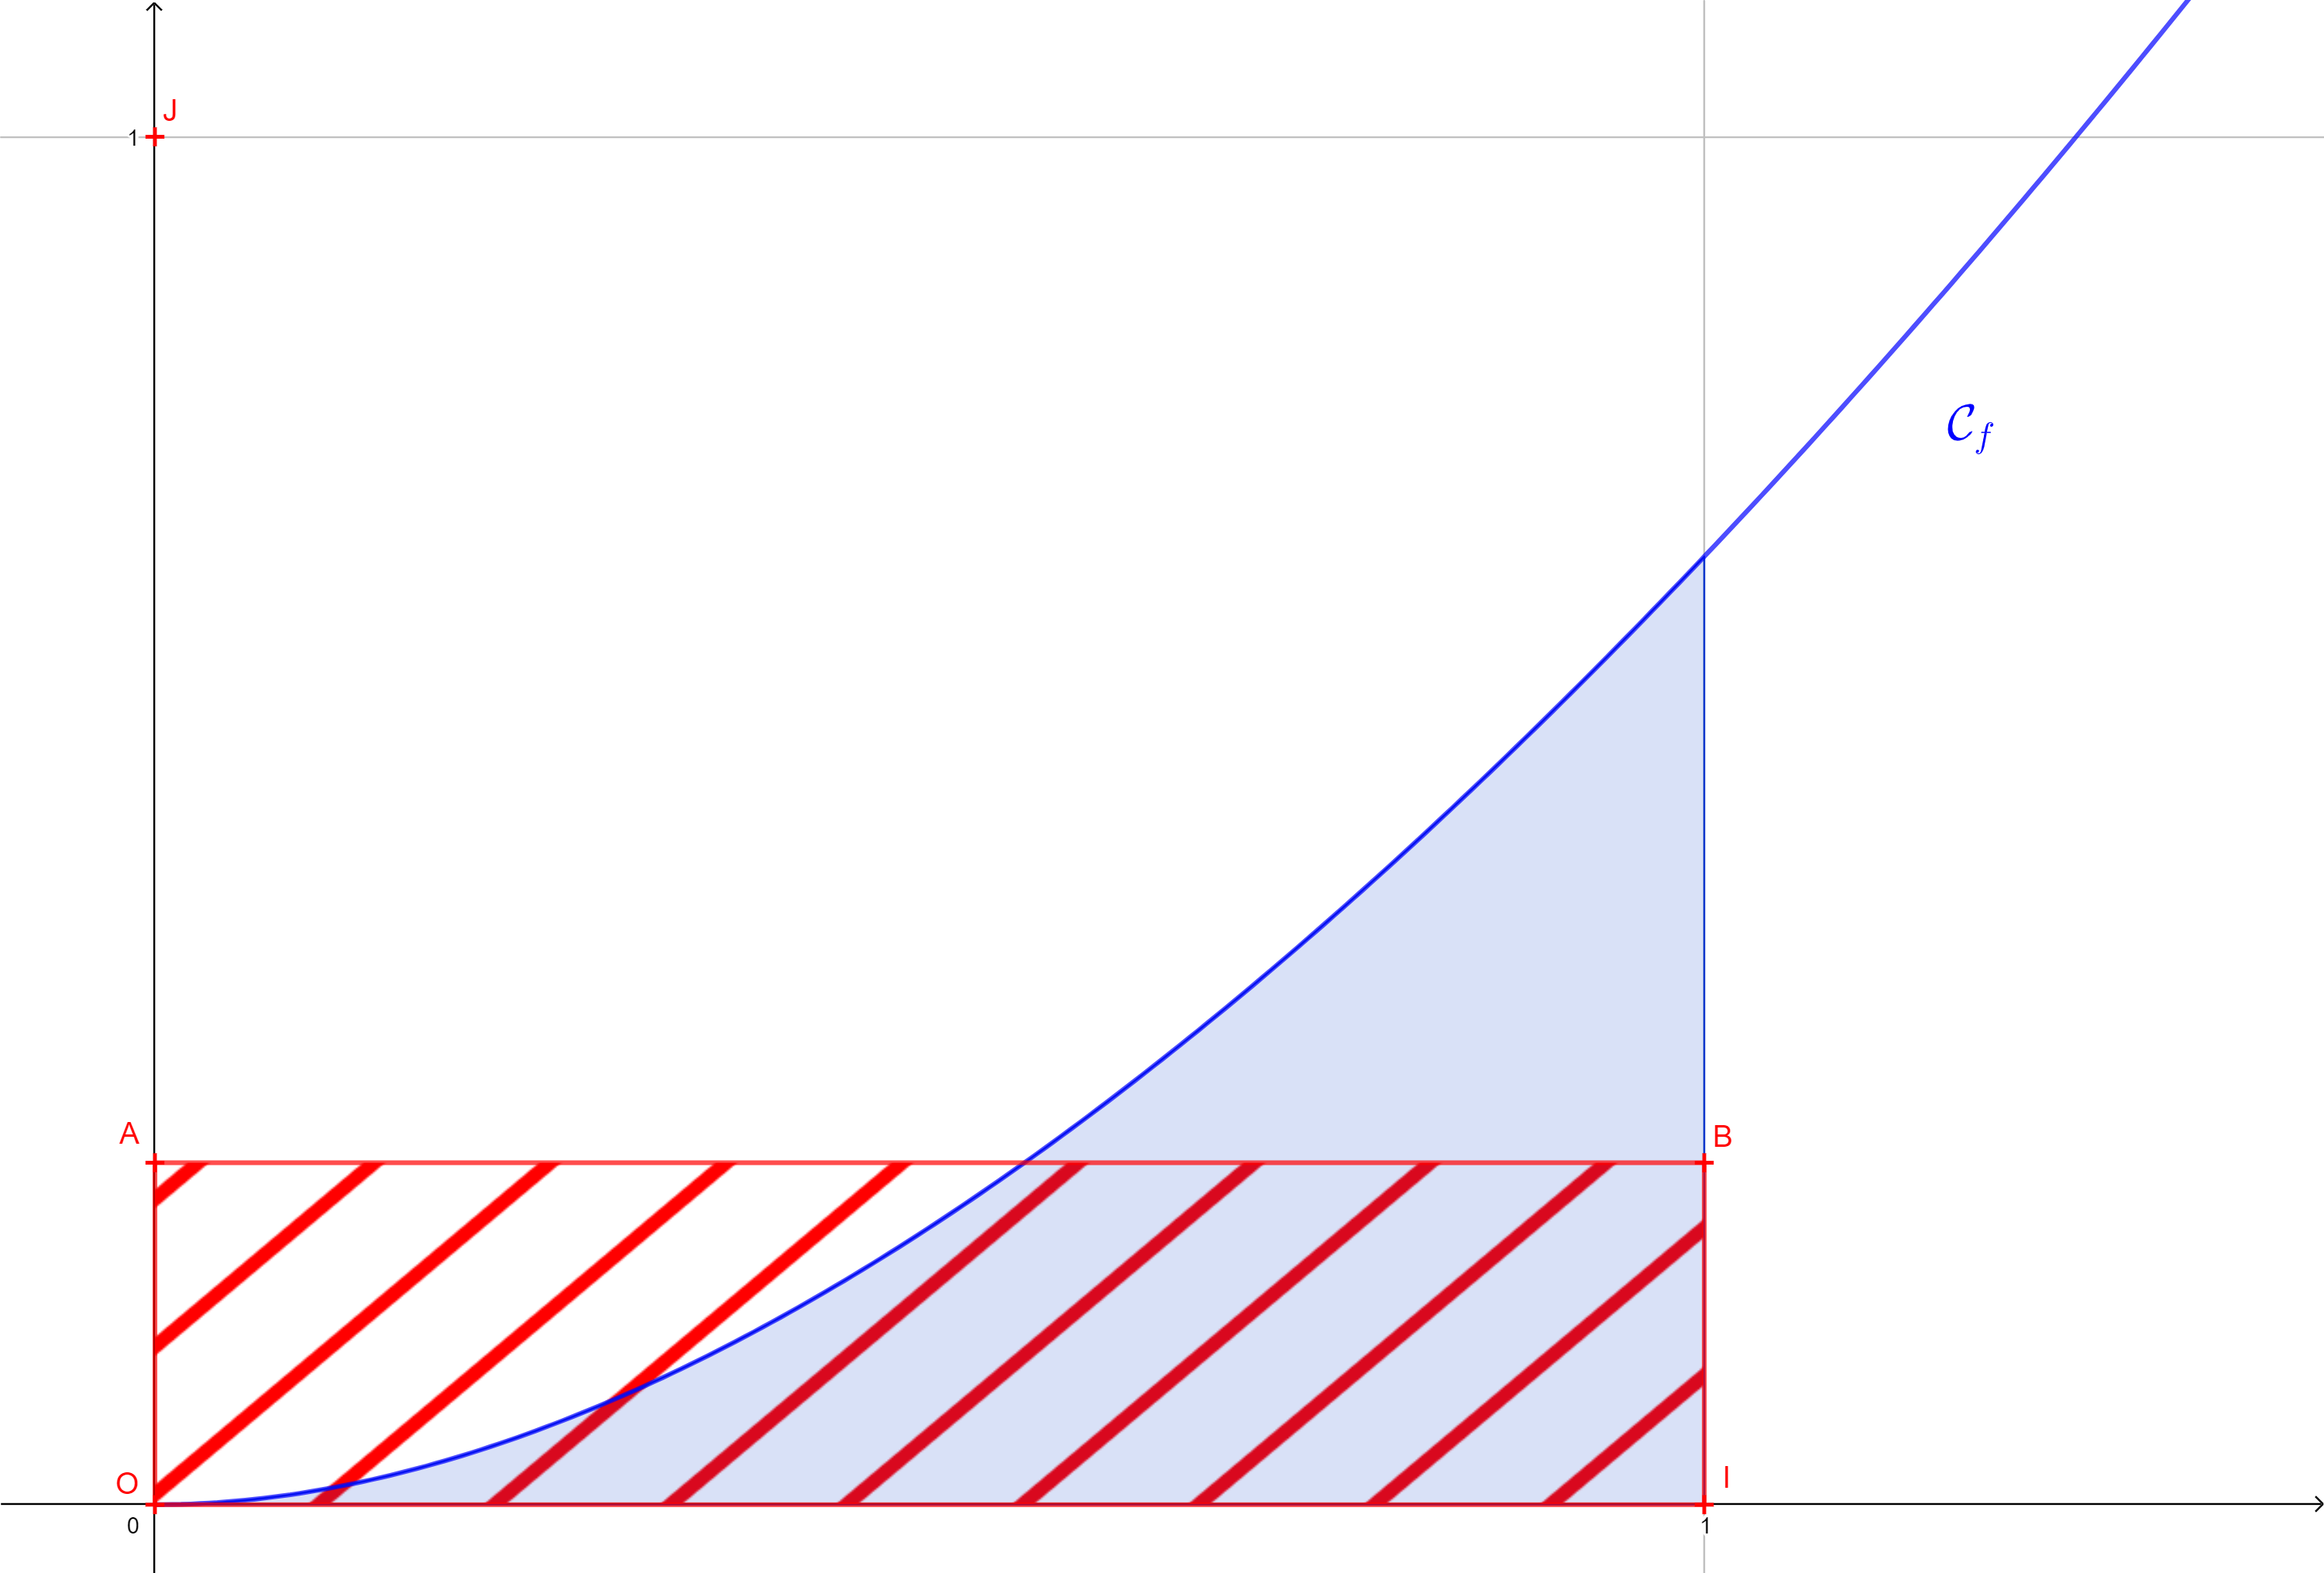
\includegraphics[width=400pt]{ControleCommunMathsGrapheExercice3}
\end{center}

% Partie A
\phantomsection
\addcontentsline{toc}{subsection}{Partie A}
\subsection*{Partie A - Etude de la fonction $f$}

% Question 1
\phantomsection
\addcontentsline{toc}{subsubsection}{Question 1}
\subsubsection*{Question 1 :}
\paragraph*{Etudier la limite de $f$ en $+\infty$\\[5mm]}

On pose $X = x + 1$ et $\displaystyle \lim_{x \to +\infty}x+1=+\infty$ donc $\displaystyle \lim_{x \to +\infty} X = +\infty$.
\\[3mm]
Ainsi, par composition : $\displaystyle \lim_{x \to +\infty}\ln{\left(x+1\right)} = \displaystyle \lim_{X \to +\infty} \ln{\left(X\right)} = +\infty$.
\\[3mm]
Donc par produit : $\displaystyle \lim_{x \to +\infty} f(x) = +\infty$.

% Question 2
\phantomsection
\addcontentsline{toc}{subsubsection}{Question 2}
\subsubsection*{Question 2 :}
\paragraph*{Etudier le sens de variations de la fonction $f$ sur $[0;+\infty[$. \\[5mm]}

$f(x) = x\ln{\left(x + 1 \right)}$ donc $f'(x) = 1 \times \ln{\left(x + 1 \right)} + x \times \frac{1}{x\ +\ 1}$.
\\[2mm]
$\forall x \in \ ]0;+\infty[$ , $x+1 > 1 \iff \ln{\left(x + 1 \right)} > 0$.
\\[2mm]
On remarque que $x > 0$ et $x + 1 >0$, de plus, la division de deux nombres positifs est elle même positive, donc $\frac{x}{x+1} > 0$.
\\[2mm]
La somme de deux nombres positifs étant positive, on peut en déduire que $f'(x)> 0$. On obtient donc :
\begin{center}
\begin{tikzpicture}
    \tkzTabInit[espcl=4, deltacl=1, lw=0.7]{$x$ /1, $f'(x)$ /1, $f(x)$ /2}{$0$, $+\infty$}
    \tkzTabLine{z,+,}
    \tkzTabVar{-/$0$,+/$+\infty$}
\end{tikzpicture}
\end{center}
Donc $f$ est strictement croissante sur $ ]0;+\infty[$ et par raisonnement similaire croissant sur $[0;+\infty[$

% Question 3
\phantomsection
\addcontentsline{toc}{subsubsection}{Question 3}
\subsubsection*{Question 3 :}
\paragraph*{Montrer que l'axe des abscisses est la tangente à $C_f$ en $x=0$ \\[5mm]}

On remarque que la droite de l'axe des abscisses à comme équation $y = 0$.
\\
L'équation de la tangente de la courbe $C_f$ représentative de $f$ en un point $a$ est : 
$y = f'(a)(x-a) + f(a)$.
\\[2mm]
On veut montrer que la tangente à la même équation que l'axe des abscisses en $x=0$ donc on prend $a=0$ et on obtient :
\\
$y = f'(0)(x-0) + f(0) = (\ln{\left( 0 + 1 \right)} + \frac{0}{0\ +\ 1})\times x + 0 \times \ln{\left( 0 + 1 \right)}= 0x + 0 = 0$
\\[2mm]
Ce qui est bien l'équation attendue de l'axe des abscisses.

% Partie B
\phantomsection
\addcontentsline{toc}{subsection}{Partie B}
\subsection*{Partie B - Calcul d'une aire}
\noindent
On pose $I = \displaystyle \int_{0}^{1} \frac{x^2}{x+1} \,dx$

% Question 1
\phantomsection
\addcontentsline{toc}{subsubsection}{Question 1}
\subsubsection*{Question 1 :}
\paragraph*{Montrer que, $\forall x \in \mathbb{R} \backslash \{-1\}$ : $\frac{x^2}{x\ +\ 1}=x-1 + \frac{1}{x\ +\ 1}$ \\[5mm]}

$
\begin{aligned}
    x-1 + \frac{1}{x+1} 
    &= \frac{(x-1)(x+1)}{x+1}+\frac{1}{x+1} \\
    &= \frac{(x-1)(x+1) + 1}{x+1} \\
    &= \frac{x^2-1+1}{x+1} \text{\hspace{3mm} d'après la troisième identité remarquable} \\
    &= \frac{x^2}{x+1}
\end{aligned}
$
\phantomsection
\addcontentsline{toc}{subsubsection}{Question 2}
\subsubsection*{Question 2 :}
\paragraph*{Montrer que $I = \ln{2} - \frac{1}{2}$.\\[5mm]}
$\begin{aligned}
    I &= \displaystyle \int_0^1 \frac{x^2}{x+1}\,dx \\
    &= \displaystyle  \int_0^1 x-1 + \frac{1}{x+1} \,dx \\
    &= \displaystyle \int_0^1 x-1 \,dx\ + \displaystyle \int_0^1 \frac{1}{x+1} \,dx \\
    &= \left[ \frac{x^2}{2}-x\right]_0^1 + \left[\ln{\left(x+1\right)}\right]_0^1 \\
    &=\frac{1}{2}-1 - \left(\frac{0}{2}-0 \right) + \ln{\left( 1+1 \right)} - \ln{\left(0+1\right)}
\end{aligned}$
\\[2mm]
Donc $I = \ln{2} - \frac{1}{2}$.

% Question 3
\phantomsection
\addcontentsline{toc}{subsubsection}{Question 3}
\subsubsection*{Question 3 :}
\paragraph*{En déduire, à l'aide d'une intégration par parties, l'aire $\mathcal{A}$, exprimée en unités d'aires (u.a.), 
du domaine entre la courbe $C_f$ et les droites d'équation $x = 0$, $x=1$ et $y=0$.\\[5mm]}

On commence par étudier le signe de $f(x)$ sur $[0;+\infty[$. 
\\
On a $x \geq 0$ et $x+1 \geq 1 \iff \ln{\left( x+1 \right)}\geq 0$ donc :
\begin{center}
\begin{tikzpicture}
    \tkzTabInit[espcl=4, deltacl=1, lw=0.7]{$x$ /1, $x$ /1, $\ln{\left(x+1\right)}$/1, $f(x)$/1}{$0$, $+\infty$}
    \tkzTabLine{z,+,}
    \tkzTabLine{z,+,}
    \tkzTabLine{z,+,}
\end{tikzpicture}
\end{center}
Donc $f(x) \geq 0$, $\forall x \in [0;+\infty[$. 
\\
Donc l'aire $\mathcal{A}$ sous la courbe $C_f$ entre 0 et 1 est l'intégrale de $f$ la fonction associée à $C_f$ entre 0 et 1.
\\
$\begin{aligned}
    \displaystyle \int_0^1 f(x) \,dx &= \displaystyle \int_0^1 x\ln{\left( x+1 \right)} \,dx \\
    &= \left[ \frac{x^2}{2} \ln{\left( x+1 \right)} \right]_0^1 - \displaystyle \int_0^1 \frac{x^2}{2} \times \frac{1}{x+1} \,dx \\
    &= \frac{1}{2}\ln{2} - 0 - \displaystyle \frac{1}{2} \int_0^1 \frac{x^2}{x+1}\,dx \\
    &= \frac{1}{2}\ln{2} - \frac{1}{2}\left( \ln{2} - \frac{1}{2} \right) \\ 
    &= - \left( -\frac{1}{2} \right) \\
    &= \frac{1}{2}
\end{aligned}$

% Partie C
\phantomsection
\addcontentsline{toc}{subsection}{Partie C}
\subsection*{Partie C - Retour au problème initial}

% Question 1
\phantomsection
\addcontentsline{toc}{subsubsection}{Question 1}
\subsubsection*{Question 1 :}
\paragraph*{Montrer que l'équation $f(x) = 0,25$ admet une unique solution  $\alpha$ sur l'intervalle $[0;1]$.\\[5mm]}

D'après la question 2 de la partie A , on sait que $f$ est strictement croissante sur $]0;+\infty[$.
\\
De plus : 
\\
\begin{itemize}
    \item[\textbullet] $ \displaystyle \lim_{x \to 0^+}f(x)=0$ \\[1mm]
    \item[\textbullet] $ \displaystyle \lim_{x \to 1}f(x) = \ln{2} $ \\[1mm]
    \item[\textbullet] D'après la question 2 de la partie A, $f$ est dérivable sur $[0;+\infty[$ et donc continue sur cette même intervalle. \\[1mm]
\end{itemize}
Donc d'après le théorème des valeurs intermédiaires, il existe une unique solution $\alpha \in [0;1]$ tel que $f(\alpha) = 0,25$, car $0,25 \in [0;\ln{2}]$.

% Question 2 
\phantomsection
\addcontentsline{toc}{subsubsection}{Question 2}
\subsubsection*{Question 2 :}
\paragraph*{Donner un encadrement de $\alpha$ à $10^{-2}$ près.\\[5mm]}

A l'aide de la calculatrice on trouve $\alpha \in [0,56;0,57]$, en effet (car $f$ est croissante): 
\\
$f(0,56) \leq f(\alpha) \leq f(0,57) \iff 0,249 \leq 0,25 \leq 0,257$ ce qui est vrai.

% Question 3
\phantomsection
\addcontentsline{toc}{subsubsection}{Question 3}
\subsubsection*{Question 3 :}
\paragraph*{Donner les points d'intersection de la courbe $C_f$ avec les côtés du rectangle OIBA dont l'aire est égale à celle du domaine bleu.\\[5mm]}

L'aire du rectangle OIBA est égale à celle de l'aire sous la courbe $C_f$ entre 0 et 1, alors que OIBA a une longueur de 1 donc sa hauteur est la valeur moyenne :
\\
$\frac{1}{1\ -\ 0}\displaystyle \int_0^1 x\ln{\left(x+1\right)} \,dx = 0,25$ donc les côtés sont délimités par $x=0$, $x=1$, $y=0$ et $y=0,25$.
\\ 
Les deux points qui appartiennent à la courbe $C_f$ et aux côtés de OIBA sont $(0;0)$ car $(0;0) = (0;f(0))$ et $y=0$, 
et $(\alpha;0,25)$ car $(\alpha;0,25) = (\alpha;f(\alpha))$, $\alpha \in[0,56;0,57]$ et $y=0,25$.

% Exercice 4
\phantomsection
\addcontentsline{toc}{section}{Exercice 4}
\section*{Exercice 4 (4 points)}

Soit $(u_n)$ la suite définie par $u_0 = 5$ et pour entier naturel $n$, \\ $u_{n+1} = 2 - e^{-u_n}$.

% Question 1
\phantomsection
\addcontentsline{toc}{subsection}{Question 1}
\subsection*{Question 1 :}

% a)
\phantomsection
\addcontentsline{toc}{subsubsection}{a)}
\paragraph*{a) Démontrer par récurrence que pour tout entier naturel,\\ $0 \leq u_{n+1} \leq u_n$\\[5mm]}

\underline{Initialisation :}
\\
$u_0 = 5$ et $u_1 = 2 - e^{-u_0} = 2 - e^{-5} \approx 1,99$ donc $0 \leq u_1 \leq u_0$ 
\\
Donc la propriété est vrai pour le rang $n = 0$.
\\
\\
\underline{Hérédité :}
\\
On suppose que $0 \leq u_{k+1} \leq u_k$ pour un certain entier naturel $k$. On souhaite montrer que $0 \leq u_{k+2} \leq u_{k+1}$.
\\ \\
Par hypothèse de récurrence on a:
\\
$ \begin{aligned}
0 \leq u_{k+1} \leq u_k 
&\iff 0 \geq -u_{k+1} \geq -u_{k} \\
&\iff 1 \geq e^{-u_{k+1}} \geq e^{-u_k} \text{ car } x \mapsto e^x \text{ est croissant sur } \mathbb{R} \\
&\iff -1 \leq - e^{-u_{k+1}} \leq - e^{-u_k} \\
&\iff 0 \leq 1 \leq 2 - e^{-u_{k+1}} \leq 2 - e^{-u_k} \\
&\iff 0 \leq u_{k+2} \leq u_{k+1} 
\end{aligned}$
\\ \\
Donc la propriété est prouvée $\forall n \in \mathbb{N}$.

% b)
\phantomsection
\addcontentsline{toc}{subsubsection}{b)}
\paragraph*{b) Que peut-on en conclure ?\\[5mm]}

On sait que $u_{n+1} \leq u_n$, $\forall n \in \mathbb{N}$ donc $(u_n)$ est décroissante, et $0 \leq u_n$, $\forall n \in \mathbb{N}$ donc $(u_n)$ est minorée. 
\\
Ainsi on en déduit que la suite $(u_n)$ est convergeante.

% Question 2
\phantomsection
\addcontentsline{toc}{subsection}{Question 2}
\subsection*{Question 2 :}

% a)
\phantomsection
\addcontentsline{toc}{subsubsection}{a)}
\paragraph*{a) Justifier que si $(u_n)$ converge, alors sa limite $l$ est solution de l'équation : $2 - e^{-x}-x=0$.\\[5mm]}

% Verifier pouquoi il est important que g est continue.
Si $(u_n)$ converge alors on pose $\displaystyle \lim_{n \to +\infty}u_n=l$ et $g$ la fonction tel que $g(u_n) = u_{n+1}$, c'est-à-dire $g(x) = 2 - e^{-x}$.
On remarque que $g'(x) = e^{-x}$ c'est-à-dire $g$ est dérivable et donc continue.
\\ \\
De plus : $\displaystyle \lim_{n \to +\infty} u_{n+1} = \displaystyle \lim_{n \to +\infty} g(u_n) = g(l)$ \\[2mm]
Par unicité de la limite d'une suite on a : $\displaystyle \lim_{n \to +\infty} u_{n+1} = \displaystyle \lim_{n \to +\infty} u_n = l$ \\[2mm]
Donc on a $\displaystyle \lim_{n \to +\infty} u_{n+1} = g(l) = l$. En particulier on a : $g(l) = l$.
\\
Alors, $g(l) = l \iff 2 - e^{-l} - l = 0$ donc $l$ est solution de l'équation $2 - e^{-x}-x=0$.

% b)
\phantomsection
\addcontentsline{toc}{subsubsection}{b)}
\paragraph*{b) On considère la fonction $f$ définie sur $[0;-\infty[$ par : $f(x)=2-e^{-x}-x$\\[5mm]}

On admet qu'elle est strictement décroissante sur $[0;+\infty[$ et que $\displaystyle \lim_{x \to +\infty}f(x)=-\infty$.
\\
Expliquer ce que calcule l'algorithme ci-dessous.
\begin{center}
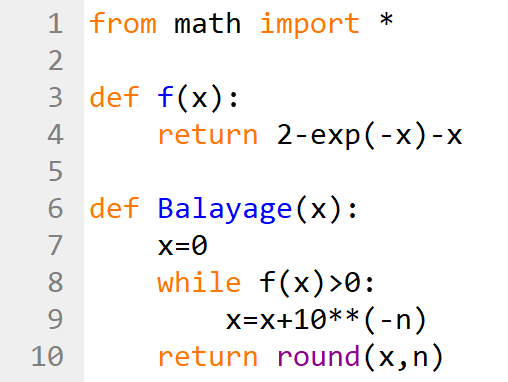
\includegraphics[width=300pt, frame]{ControleCommunMathsCodeExercice4.png}
\end{center}
On vérifie les valeurs prises par $f(x)$ pour $x$ partant de 0 et augmentant en incréments de $10^{-n}$. 
$f'(x)=e^{-x}-1$, c'est-à-dire $f$ est dérivable et donc continue. 
On sait que $f(0) = 1$ et $\displaystyle \lim_{x \to +\infty}f(x) = -\infty$ et que 
$f(x)$ est strictement décroissant donc d'après le théorème des valeurs intermédiaires il existe une unique solution $\alpha$ tel que $f(\alpha)=0$. 
\\[2mm]
Comme la fonction est décroissante et $f(0)>0$, on sait qu'elle va franchir la valeur de 0 et ensuite être négative, l'algorithme vérifie donc la première valeur de $x$ 
pour laquelle $f(x)<0$ ce qui approxime $\alpha$. 
\\[2mm]
On remarque que la valeur donnée par l'algorithme est la solution arrondi par l'excès à $10^{-n}$ près de l'équation $f(x)=0$ ainsi que la limite de $(u_n)$

% c)
\phantomsection
\addcontentsline{toc}{subsubsection}{c)}
\paragraph*{c) Quel résultat obtient-on pour $n=2$ ?\\[5mm]}

D'aprés ce programme, pour $n=2$, la valeur renvoyée est $1,85$. 
\\
En effet $f(1,84) \approx 0,0011 >0$ et $f(1,85) \approx -0,0072 < 0$ donc 1,85 est bien la première valeur (par incréments de 0,01 ou $10^{-2}$) pour laquelle $f(x)$ est négative.

\newpage
\pagenumbering{roman}
\tableofcontents
\end{document}

% Notes 

% https://tex.stackexchange.com/questions/33443/box-around-single-element-in-list
% https://tex.stackexchange.com/questions/407790/equation-block-alignment-to-the-left